\section*{Systemets virkemåte}
\setcounter{section}{3}
\addcontentsline{toc}{section}{Systemets virkemåte}

\setcounter{subsection}{0}

\begin{figure}[H]
    \centering
    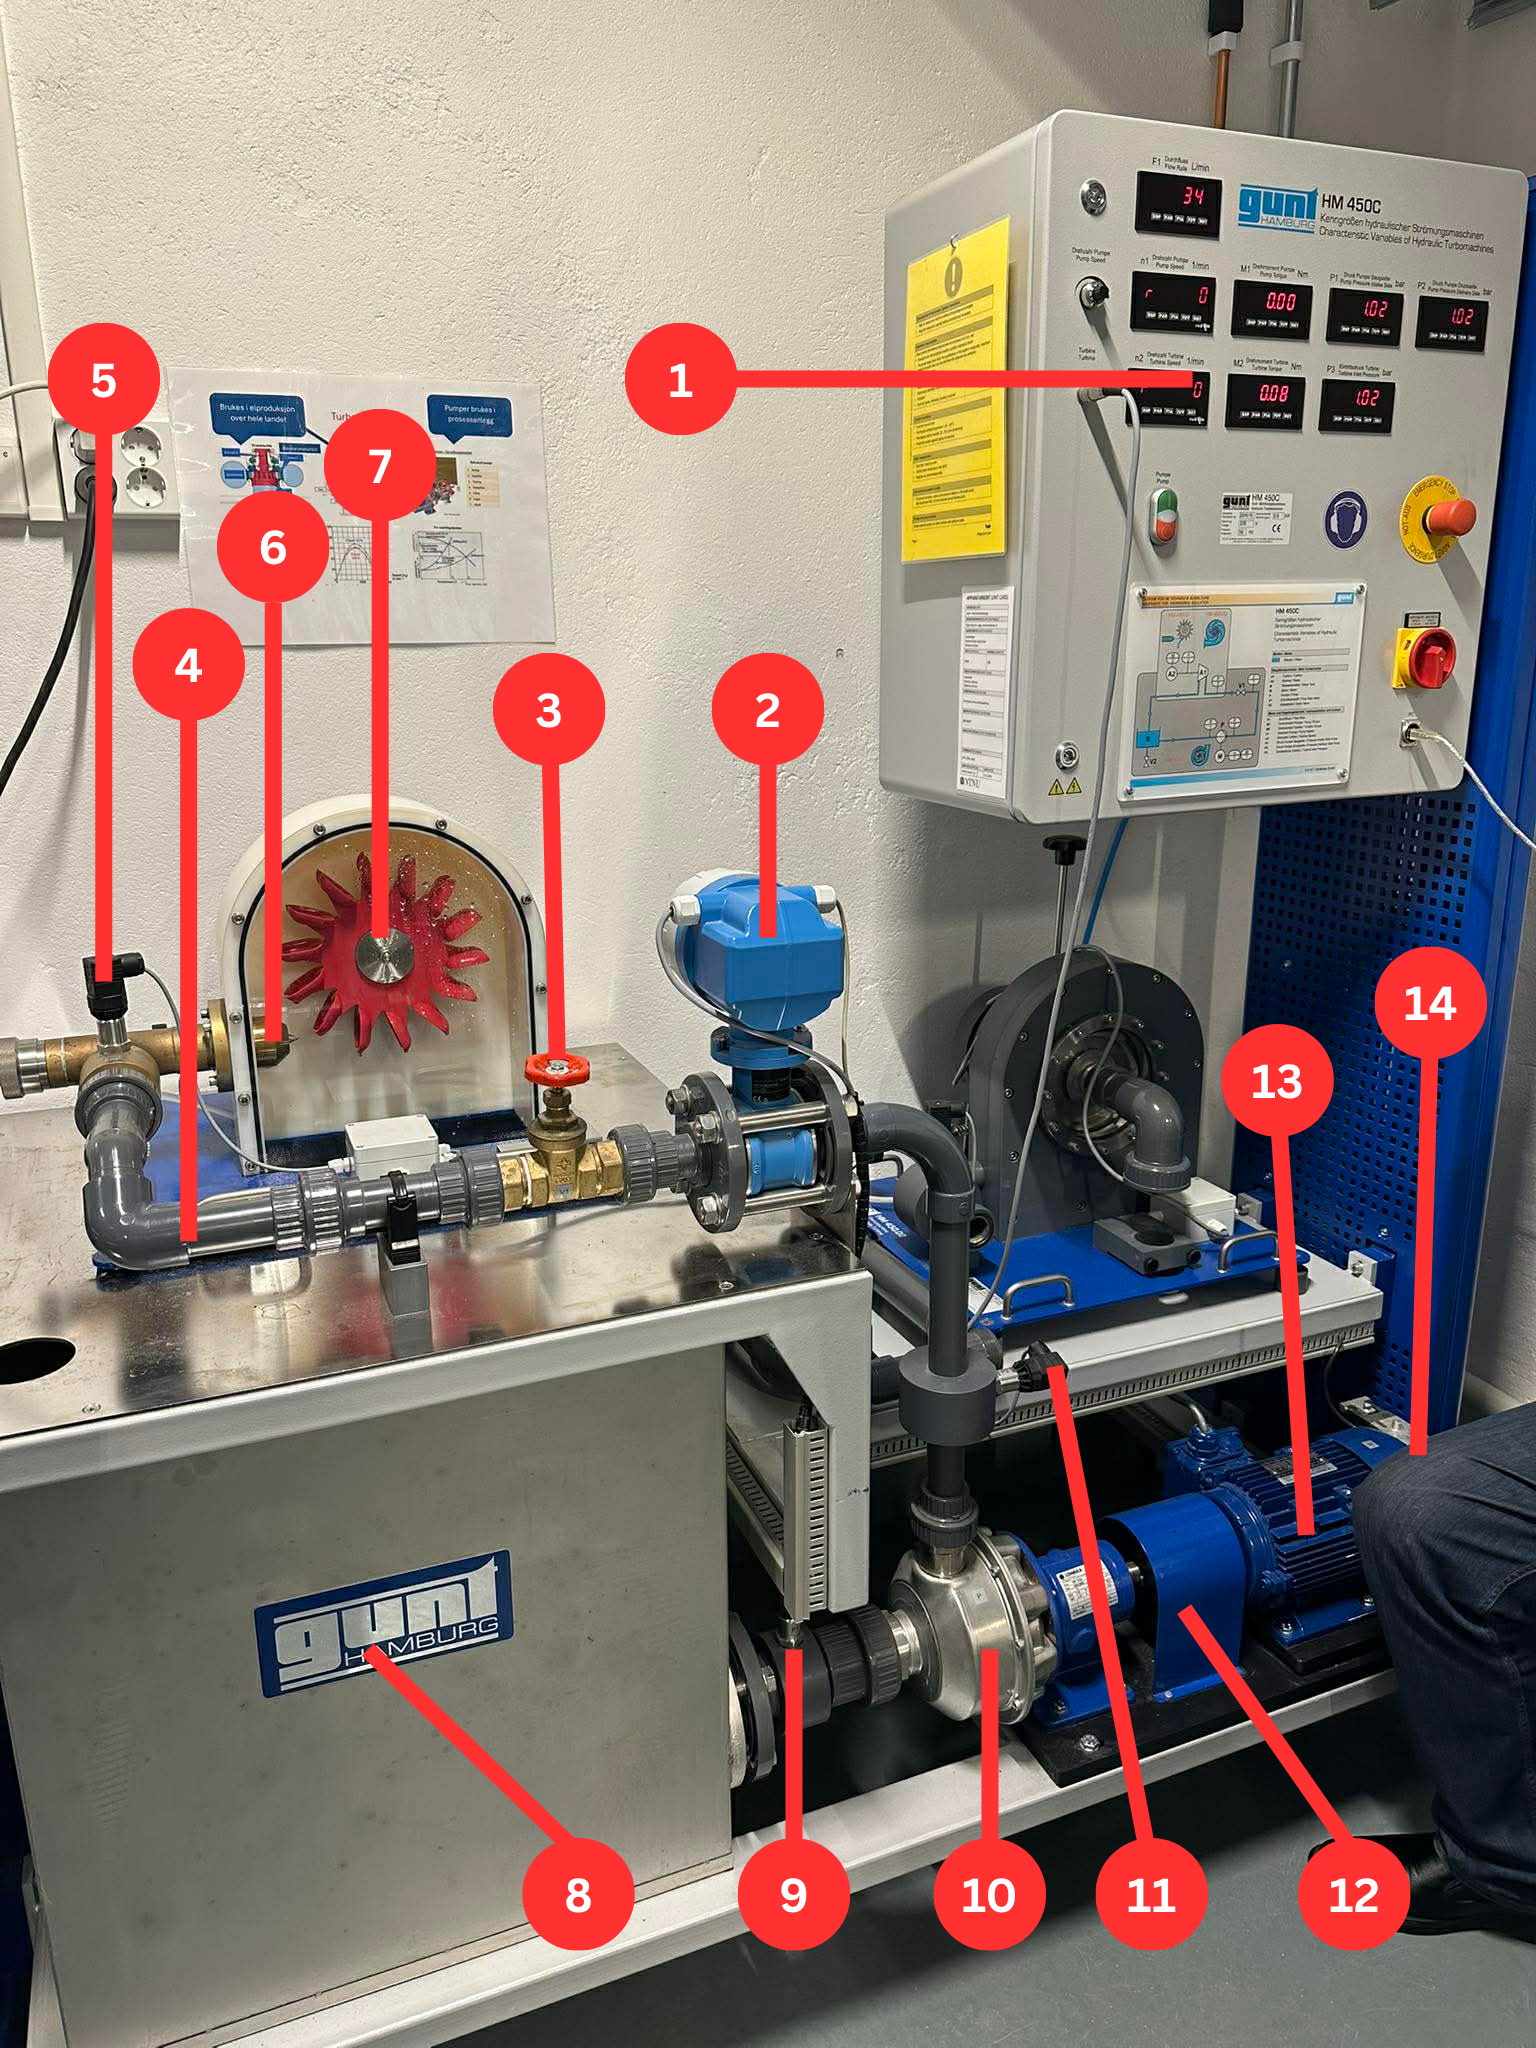
\includegraphics[width=0.5\linewidth]{Ny_lab-oppsett.png}
    \caption{Lab-oppsettet for Pelton-turbin. Nummereringen refererer til hovedkomponentene beskrevet i teksten}
    \label{fig:lab}
\end{figure}


Oppsettet er et lukket vannkretsløp. Pumpen (10) sender vann gjennom tilførselsrøret (4) til dysen (6), som retter en vannstråle mot turbinen (7). Belastningen reguleres med bremsereimen, og turtall, dreiemoment, volumstrøm og trykk avleses direkte fra oppsettet. Etter at vannet har truffet turbinen faller det tilbake til tanken (8), og kretsløpet gjentas.